\chapter{Preliminares}\label{ch:Preliminares}
\section{Historia de la epidemiología}\label{sec:Historia de la epidemiología}
De acuerdo con \cite{epiDictionary}, la epidemiología se encarga de estudiar la ocurrencia y distribución de eventos, estados y procesos relacionados con la salud de distintas poblaciones, con el objetivo de brindar estrategias de control y prevención de problemas de salud relevantes.

El primer intento por modelar teóricamente la propagación de una enfermedad, fue realizado por Daniel Bernouilli en 1760, en el cual, basándose en sus conocimientos en medicina y matemáticas, desarrolló un modelo que describe el comportamiento de la viruela y evalúa el impacto teórico de la inoculación para su época \cite{shortHistory}. 

Sin embargo, en el modelamiento epidemiológico se considera como punto de partida el modelo descrito por Kermack y McKendrick en 1927, también conocido como modelo SIR, en el que se establecen relaciones entre tres estados de una enfermedad (Susceptible-Infectado-Recuperado) y se implementan los conceptos de tasa de contagio y de recuperación \cite{malariaSIR}. Desde entonces se han desarrollado múltiples variaciones sobre el modelo SIR, con el objetivo de analizar diferentes tipos de enfermedades de una manera más precisa, considerando por ejemplo diferentes estados, tasas de natalidad y mortalidad, entre otros \cite{diego2010}.

Por otra parte y debido a los avances tecnológicos de las últimas décadas, se han desarrollado modelos y simulaciones que permiten analizar características que no eran posibles con los modelos anteriormente mencionados. Por ejemplo, patrones de movilidad \cite{colaGNN, epidemiologicalNeuralNetwork}, disminución en la cantidad de contagios debido a un aislamiento preventivo \cite{stayHome}, contagios de individuo a individuo \cite{heterogeneousPopulation} e interacciones en masa \cite{combiningGraph, transfer2021}, la mayoría realizadas con una fuerte influencia de las redes neuronales y complejas, apoyadas fuertemente sobre la teoría de grafos.

\section{Estudio epidemiológico}\label{sec:Estudio epidemiológico}
Uno de los objetos de estudio con mayor importancia en el campo de la epidemiología es la cualidad endémica de la enfermedad, es decir, si la enfermedad afectará a la población por un largo periodo de tiempo o si desaparecerá gradualmente. La manera en la que se determina está capacidad está dada por los siguientes indicadores:

\begin{itemize}
    \item \textbf{Número básico de reproducción $R_0$:} Se define como la cantidad de individuos que infecta el paciente cero en una población completamente susceptible. En general, si $R_0<1$ la enfermedad desaparecerá paulatinamente y sí $R_0>1$, podríamos estar ante un caso de endemia.
    \item \textbf{Número de contactos adecuados $\sigma(t)$:} Es la cantidad de contactos con individuos del sistema que realiza un individuo infectado durante su etapa de infección, cuando se introduce en la población en el momento $t$.
    \item \textbf{Número de desplazamiento $R(t)$:} Se entiende como la cantidad promedio de infecciones secundarias que produce un individuo infectado durante su etapa de infección, cuando es introducido en la población en el momento $t$. De ese modo, $R(t) = \sigma(t)\cdot S(t)$, donde $S(t)$ indica la cantidad de individuos susceptibles en el momento $t$.
\end{itemize}

Heesterbeek y Dietz definen el número básico de reproducción $R_0$ como
\begin{equation}\label{eq:R0}
    R_0 = \int_0^\infty b(a)F(a) da
\end{equation}
donde $b(a)$ representa la cantidad promedio de nuevos contagios que producirá un individuo infectado durante un tiempo y $F(a)$, conocida como la función de supervivencia, representa la probabilidad de que un individuo recién infectado se mantenga en ese estado durante al menos un tiempo $a$ \cite{conceptOfR0, perspectivesOnR0}.

\section{Modelos epidemiológicos clásicos}\label{sec:Modelos epidemiológicos clásicos}

Tradicionalmente, se han utilizado modelos de compartimientos para elaborar análisis epidemiológicos. En estos modelos, cada individuo perteneciente a la población de estudio es clasificado en uno de $n$ posibles estados, según su estado de salud.

Las siglas de cada estado del modelo definen su nombre, por ejemplo, el modelo MSEIR define la interacción entre poblaciones con inmunidad "pasiva" o temporal (M), en donde la inmunidad de los individuos se genera a partir de los anticuerpos heredados de la madre. Con la desaparición de los anticuerpos, estos individuos se vuelven susceptibles a contraer la enfermedad (S). Si un individuo susceptible entra en contacto con un individuo infectado, pasará al estado de exposición (E) en donde ya se considera infectado pero incapaz de transmitir la enfermedad. En el momento en el que el individuo adquiera la capacidad de contagiar la enfermedad, se pasará al estado (I) y finalmente, cuando el individuo se recupere y adquiera inmunidad, pasará al estado (R) del modelo.\cite{modelCompartimental}

\begin{figure}[h]
  \centering
    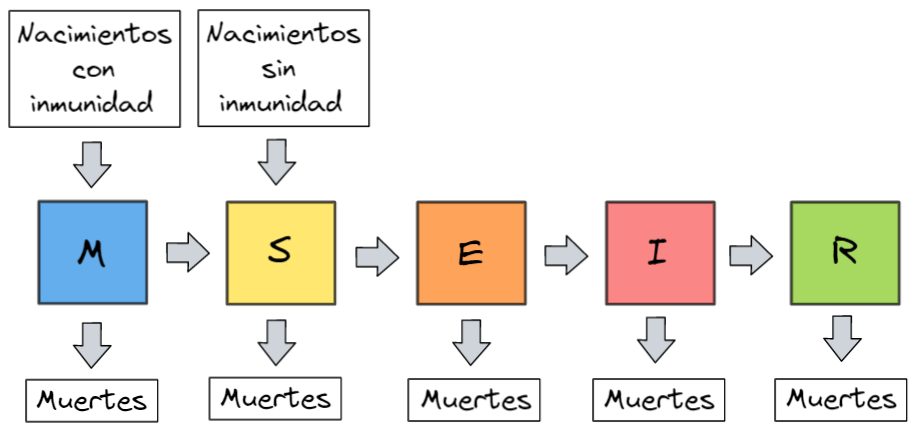
\includegraphics[width=0.7\textwidth]{Imagenes/MSEIR_compatimientos.PNG}
  \caption{Diagrama de compartimientos para el modelo MSEIR}
  \label{fig:diagrama MSEIR}
\end{figure}

Generalmente cuando hablamos de modelos epidemiológicos se consideran tres estados o clases en las que podemos dividir a la población en el tiempo: Los que pueden contraer la enfermedad, los que se infectan y los que se recuperan. Si los que se recuperan no adquieren una inmunidad permanente, nos encontraremos ante un modelo SIS, en el que los susceptibles pueden contraer la enfermedad y una vez se recuperan vuelven al estado de susceptibilidad. Por otro lado, si los individuos que se recuperan generan inmunidad a la enfermedad, estaremos ante un modelo SIR. 

Teniendo en cuenta este tipo de consideraciones nos permitimos establecer a los modelos SIS y SIR como foco principal de nuestra investigación sin dejar a un lado la idea de retomar modelos como el MSEIR para investigaciones futuras. Adicionalmente para efectos aplicables consideraremos las variaciones que tienen en cuenta la natalidad y mortalidad bien sea a causa o por efectos ajenos a la enfermedad.

Brauer y Castillo describen en \cite{mateModelsInPopulationAndEpidemiology} los planteamientos y técnicas para analizar este tipo de modelos. Nos apoyaremos también en el trabajo realizado por Diego de Pereda Sebastián en \cite{diego2010} para algunos resultados y observaciones interesantes sobre cada modelo.

\subsection{El modelo SIS}\label{sub:El modelo SIS}

El modelo SIS considera 2 posibles estados, susceptibles (S) e infectados (I). Las variaciones entre los estados vienen dadas por los nuevos contagios y los individuos que se recuperan de la enfermedad. Adicionalmente, cada estado se ve afectado por los parámetros que describen la natalidad/mortalidad y la muerte a cauda de la enfermedad. 

Los diferentes estados del modelo se pueden apreciar en el diagrama (\ref{fig:diagrama SIS}):

\begin{figure}[h]
  \centering
    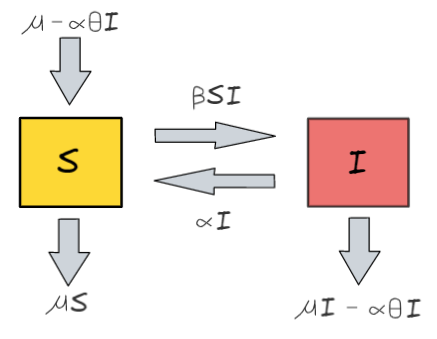
\includegraphics[width=0.4\textwidth]{Imagenes/SIS_compartimientos.PNG}
  \caption{Diagrama de compartimientos para el modelo SIS}
  \label{fig:diagrama SIS}
\end{figure}

Es importante recordar que trabajaremos sobre una población de tamaño constante y normalizado, por lo que $S + I = 1$ y en consecuencia $S' + I' = 0$.

Normalmente cuando se habla de modelos epidemiológicos con muerte por enfermedad se consideran 4 parámetros: 

\begin{itemize}
    \item La \textbf{tasa de infección $\beta$}, que representa la probabilidad que tiene un individuo susceptible de adquirir la enfermedad luego de un contagio con un infectado.
    \item La \textbf{tasa de recuperación $\alpha$}, que podemos entender como la probabilidad de que un infectado se recupere de la enfermedad.
    \item La \textbf{tasa de natalidad/mortalidad $\mu$}, que en el caso de los modelos clásicos se considera igual. La natalidad nos indica la cantidad de individuos que ingresan al espacio y la mortalidad representa los individuos que fallecen por causas ajenas a la enfermedad.
    \item La \textbf{tasa de muerte por enfermedad $\theta$}, que nos indica la probabilidad que tiene un infectado de fallecer a causa de la enfermedad.
\end{itemize}

Podemos describir el modelo a partir de un sistema de ecuaciones diferenciales como sigue:

\begin{equation}\label{eq:Modelo SIS}
\left\{
\begin{array}{l}
S' = \mu(1 - S) + (1 - \theta)\alpha I - \beta S I \\
I' = \beta S I - (1 - \theta)\alpha I - \mu I
\end{array}
\right.
\end{equation}

Para determinar los escenarios bajo los cuales una enfermedad es endémica debemos calcular el valor de $R_0$ para nuestro sistema de ecuaciones diferenciales (\ref{eq:Modelo SIS}). Recuerde que para determinar el valor de $R_0$ se considera una población completamente susceptible, es decir, $S=1$ y $I=0$.

Observe que los nuevos infectados vienen dados por el término $\beta S$, con lo cual definimos $b(t) = \beta S = \beta$. Por otro lado, los flujos que determinan la salida del estado de infección de los individuos viene dado por los términos $-\alpha(1-\theta)I-\mu I$, de modo que si llamamos $I(t)$ a la cantidad de individuos infectados que permanecieron infectados desde el momento 0, tenemos

\begin{equation}\label{eq:Cambio en I}
\frac{dI}{dt} = -\alpha(1-\theta)I-\mu I
\end{equation}

Donde al usar el método de separación de variables obtenemos

\begin{equation}\label{eq:Infectados en el tiempo}
I(t) = I(0)e^{-(\alpha(1-\theta)+\mu)t}
\end{equation}

De ese modo, podemos afirmar que la proporción de individuos que permanecen infectados hasta un tiempo $t$ viene dado por $e^{-(\alpha(1-\theta)+\mu)t}$, con lo cual $F(t)=e^{-(\alpha(1-\theta)+\mu)t}$. Finalmente, al reemplazar en (\ref{eq:R0}) obtenemos:

\begin{align*}
R_0 &= \lim_{T\to\infty}\int_0^T b(t)F(t) dt \\
&= \lim_{T\to\infty}\int_0^T \beta e^{-(\alpha(1-\theta)+\mu)t} dt\\
&= \frac{\beta}{\alpha(1-\theta)+\mu}
\end{align*}

\underline{\textit{Observación:}} De la ecuación (\ref{eq:Infectados en el tiempo}) podemos afirmar que la cantidad de individuos infectados tiende a cero cuando $t$ tiende a infinito.

\subsubsection{Análisis de estabilidad}

Para analizar la estabilidad de nuestro modelo SIS debemos conocer sus puntos de equilibrio. Al anular ambas derivadas nos damos cuenta de que están dados por 

$$P_0=(S_a,I_a)=(1,0), P_1=(S_b,I_b)=\left(\frac{\alpha(1-\theta)+\mu}{\beta},\frac{\beta-\alpha(1-\theta)-\mu}{\beta}\right)$$

Veamos que los puntos de equilibrio satisfacen las condiciones de ser positivos y menores o iguales a 1:

En el caso de $P_0$ la verificación es trivial. Por otro lado, para el caso de $P_1$ observe que 

$$0\leq\alpha(1-\theta)+\mu\leq\beta \longrightarrow \frac{\alpha(1-\theta)+\mu}{\beta}\text{, }\frac{\beta+\alpha(1-\theta)+\mu}{\beta}\geq0$$

Si dividimos la expresión del lado izquierdo por $\beta$ obtenemos

$$0\leq \frac{\alpha(1-\theta)+\mu}{\beta}\leq1$$

De donde podemos afirmar que 

$$1-\frac{\alpha(1-\theta)+\mu}{\beta}\leq1 \longrightarrow \frac{\beta-\alpha(1-\theta)-\mu}{\beta}\leq1$$

De donde podemos concluir que ambos puntos de equilibrio cumplen las condiciones de tener coordenadas positivas y menores que la unidad.

Es momento de determinar los comportamientos que describen ambos puntos, $P_0$ y $P_1$. Consideremos el jacobiano de nuestro modelo:

$$|A-\lambda I|=
\left|\begin{array}{cc}
-\mu-\beta I-\lambda & \lambda(1-\theta)-\beta S \\
\beta I & \beta S-\alpha(1-\theta)-\mu-\lambda
\end{array}\right|$$

Si evaluamos en $P_0$ obtendremos los valores propios

$$\left\{\begin{array}{l}\lambda=-\mu \\
\lambda=\beta-\alpha(1-\theta)-\mu\end{array}\right.$$

Con lo cual, podemos afirmar que si $R_0>1$, $P_0$ se comportará como un punto de silla y por otro lado, si $R_0<1$ estaremos ante un nodo estable. Para el caso de $P_1$ tendremos un comportamiento tipo sumidero dado que $\lambda=0,\lambda=-\mu$ son los valores propios asociados a $P_1$.

\subsubsection{Estudio numérico}

Para representar las soluciones del sistema de ecuaciones diferenciales que describe el modelo SIS usaremos el método de Euler, el cual se implementó en el módulo: "\textit{CompartmentalModelsInEDOS}".

De manera general, dadas unas condiciones iniciales $S(0)=S_0,I(0)=I_0$ aplicamos el método de Euler a partir de la siguiente expresión

$$\left\{\begin{array}{l}
S_{t+1} = S_t + h\cdot(\mu(1 - S_t) + (1 - \theta)\alpha I_t - \beta S_t I_t ) \\
I_{t+1} = I_t + h\cdot(\beta S_t I_t - (1 - \theta)\alpha I_t - \mu I_t)
\end{array}\right.$$

\begin{itemize}
    \item Consideremos por ejemplo una enfermedad en la que la tasa de recuperación $\alpha$ es del $0.2$ y su tasa de infección es de $\beta=0.5$ con una tasa de letalidad de $\theta=0.4$. La tasa de natalidad para nuestra población será de $\mu=\frac{1}{75\cdot365}$, es decir, una esperanza de vida de $75$ años.
    
    \begin{figure}[h]
      \centering
        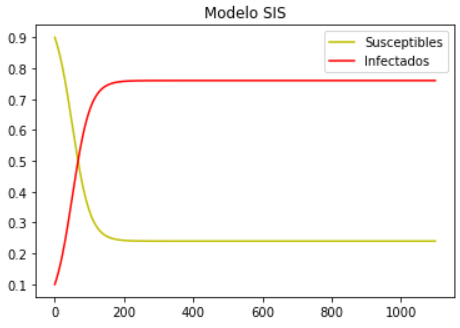
\includegraphics[width=0.4\textwidth]{Imagenes/ex1SIS.PNG}
      \caption{Evolución de la enfermedad en 1100 días con $S_0=0.9,I_0=0.1$ y $h=0.1$.}
      \label{fig:Ejemplo 1 - SIS}
    \end{figure}
\end{itemize}

\subsection{El modelo SIR}\label{sub:El modelo SIR}

Para este modelo se considera el estado de inmunidad frente a la enfermedad R. A diferencia del modelo SIS, en el modelo SIR no hay una interacción del estado I al estado S, ya que se supone que los individuos que se recuperen de la enfermedad no podrán volver a contraerla, por lo que pasaran al estado R. 

En el diagrama (\ref{fig:diagrama SIR}) se pueden apreciar las interacciones para los estados del modelo:

\begin{figure}[h]
  \centering
    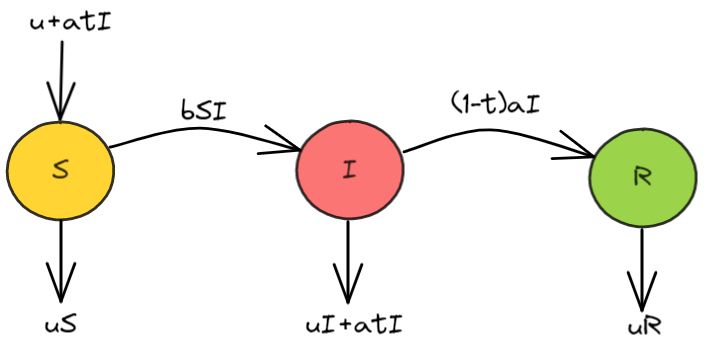
\includegraphics[width=0.7\textwidth]{Imagenes/SIR_compartimientos.PNG}
  \caption{Diagrama de compartimientos para el modelo SIR}
  \label{fig:diagrama SIR}
\end{figure}

De ese modo, el sistema de ecuaciones diferenciales que describe las interacciones entre estados viene dado por la siguiente ecuación:

\begin{equation}\label{eq:Modelo SIR}
\left\{
\begin{array}{l}
S' = \mu(1 - S) + \alpha\theta I - \beta S I \\
I' = \beta S I - \mu I - \theta\alpha I - (1 - \theta)\alpha I = \beta S I - \alpha I - \mu I \\
R' = \alpha I - \alpha\theta I - \mu R
\end{array}
\right.
\end{equation}

En este caso, la ecuación diferencial que describirá la cantidad de individuos infectados desde el momento 0 viene dada por:

\begin{equation}\label{eq:Infectados en el tiempo I - SIR}
    \frac{dI}{dt}=-\mu I - \alpha I \longrightarrow I(t)=I(0)e^{-(\alpha+\mu)t}
\end{equation}

Con lo que definimos $F(t)=e^{-(\alpha+\mu)t}$. Por otra parte, la función $b(t)$ estará definida de la misma manera que en el modelo SIS debido a la manera en la que se describe el modelo. Así, al reemplazar en (\ref{eq:R0}):

\begin{align*}
R_0 &= \int_0^\infty b(t)F(t) dt \\
&= \lim_{T\to\infty} \int_0^T b(t)F(t) dt \\
&= \frac{\beta}{\alpha+\mu}
\end{align*}

\underline{\textit{Observación:}} De acuerdo con la ecuación \ref{eq:Infectados en el tiempo I - SIR}, la población de infectada tendera a cero cuando $t$ tienda a infinito.

\subsubsection{Análisis de estabilidad}

Al igualar a cero las derivadas del sistema de ecuaciones \ref{eq:Modelo SIR} obtenemos los puntos de equilibrio:

$$\begin{array}{cc}
P_0=(S_a,I_a,R_a)=(1,0,0) & P_1=(S_b,I_b,R_b)=\left(\frac{\alpha+\mu}{\beta},\frac{\mu(\beta-\alpha-\mu)}{\beta(\mu+(1-\theta)\alpha)},\frac{(1-\theta)\alpha(\beta-\alpha-\mu)}{\beta(\mu+(1-\theta)\alpha)}\right)
\end{array}$$

Veamos que las coordenadas de ambos puntos cumplen las condiciones de ser positivos y menores o iguales que uno: 

En el caso de $P_0$ se cumple de manera trivial. Por otro lado, como $\alpha,\beta,\theta$ y $\mu$ son valores positivos podemos afirmar que $S_b>0$, para $I_b$ y $R_b$ observe que 

$$\begin{array}{ccc}
\frac{\mu(\beta-\alpha-\mu)}{\beta(\mu+(1-\theta)\alpha)},\frac{(1-\theta)\alpha(\beta-\alpha-\mu)}{\beta(\mu+(1-\theta)\alpha)}>0 & \text{, si} & \beta-\alpha-\mu>0
\end{array}$$

De la ecuación anterior podemos afirmar que 

$$\beta-\alpha-\mu>0\longrightarrow1>\frac{\alpha+\mu}{\beta}$$

Además, como ya sabemos que se trata de un valor positivo podemos deducir que 

\begin{align*}
1&>1-\frac{\alpha+\mu}{\beta} \\
&= \frac{(\beta-\alpha-\mu)(\mu+(1-\theta)\alpha)}{\beta(\mu+(1-\theta)\alpha)}\\
&= \frac{\mu(\beta-\alpha-\mu)}{\beta(\mu+(1-\theta)\alpha)}+\frac{(1-\theta)\alpha(\beta-\alpha-\mu)}{\beta(\mu+(1-\theta)\alpha)}
\end{align*}

Con lo cual,

$$\frac{\mu(\beta-\alpha-\mu)}{\beta(\mu+(1-\theta)\alpha)},\frac{(1-\theta)\alpha(\beta-\alpha-\mu)}{\beta(\mu+(1-\theta)\alpha)}<1$$

Hemos demostrado que ambos puntos de equilibrio cumplen con las condiciones de tener coordenadas positivas y menores a la unidad. Ahora analizaremos la estabilidad de nuestro modelo SIR, consideremos el jacobiano de nuestro sistema de ecuaciones diferenciales:

$$|A-\lambda I|=(-\mu-\lambda)
\left|\begin{array}{cc}
-\beta I-\mu-\lambda & -\beta S+\theta\alpha\\
\beta I & \beta S-\alpha-\mu -\lambda
\end{array}\right|$$

Si evaluamos en el punto $P_1$, podemos identificar un comportamiento de tipo silla si $\beta-\alpha-\mu>0$, en caso contrario nos encontraremos ante un nodo estable.

Si tomamos ahora el punto $P_2$ y observamos los valores propios 

$$\left\{\begin{array}{l}
\lambda=-\mu\\
\lambda=-\frac{1}{2}\frac{\mu\beta-\mu\theta\alpha+\sqrt{(\mu\beta-\mu\theta\alpha)^2-4\mu(\beta-\alpha-\mu)(\alpha+\mu-\theta\alpha)^2}}{\alpha+\mu-\theta\alpha} \\
\lambda=-\frac{1}{2}\frac{\mu\beta-\mu\theta\alpha-\sqrt{(\mu\beta-\mu\theta\alpha)^2-4\mu(\beta-\alpha-\mu)(\alpha+\mu-\theta\alpha)^2}}{\alpha+\mu-\theta\alpha}
\end{array}\right.$$

Y de ese modo obtendremos dos tipos de comportamientos, una espiral estable si los valores propios son imaginarios y un nodo estable en el caso de que los valores propios sean reales.

\subsubsection{Estudio numérico}

De manera general, si usamos el método de Euler dadas las condiciones iniciales $S(0)=S_0,I(0)=I_0$ las expresiones que describen las soluciones discretas son:

$$\left\{\begin{array}{l}
S_{t+1} = S_t + h\cdot(\mu(1 - S_t) + \alpha\theta I_t - \beta S_t I_t) \\
I_{t+1} = I_t + h\cdot(\beta S_t I_t - \alpha I_t - \mu I_t) \\
R_{t+1} = R_t + h\cdot(\alpha I_t - \alpha\theta I_t - \mu R_t)
\end{array}\right.$$

\begin{itemize}
    \item Para este ejemplo supondremos una variación de la enfermedad contemplada en el ejemplo del modelo SIS en la que los individuos que se recuperan de la enfermedad adquieren inmunidad.
    
    \begin{figure}[h]
      \centering
        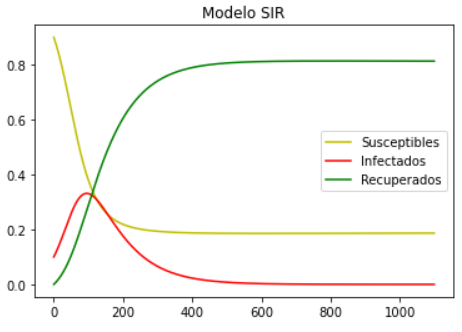
\includegraphics[width=0.4\textwidth]{Imagenes/ex1SIR.PNG}
      \caption{\centering Evolución de la enfermedad en 1100 días con $S_0=0.9,I_0=0.1,R_0=0$ y $h=0.1$.}
      \label{fig:Ejemplo 1 - SIR}
    \end{figure}
\end{itemize}

\section{Autómatas celulares}\label{sec:Autómatas celulares}

Los autómatas celulares nacen con el trabajo de Von Neumann a finales de la década de 1940 con su trabajo \textit{"The
General and Logical Theory of Automata"} en el que se plantean por primera vez las ideas para una máquina capaz de autorreplicarse. Trabajó sobre un sistema bidimensional discreto para desarrollar dinámicas bastante complejas que además fueran autorreplicables \cite{alfons2010,ACaplicacionesComputacion}.

De acuerdo con \cite{descripcionyAplicaciones}, podemos pensar en un autómata celular como un conjunto de células que tienen diferentes comportamientos en el tiempo y que interactúan entre sí, de la misma manera que en sistema biológico de donde se obtiene su nombre.

La implementación computacional de un autómata celular por lo general se hace sobre matrices, por lo que el sistema que se quiere modelar se describe sobre una malla de tamaño regular, como en la figura (\ref{fig:AC a matriz}). Una vez se define el significado de cada célula se establece una equivalencia con un conjunto de valores o caracteres que conoceremos como estados del autómata y finalmente, sobre esos estados definiremos las reglas de comportamiento para nuestro modelo.

\begin{figure}[h]
  \centering
    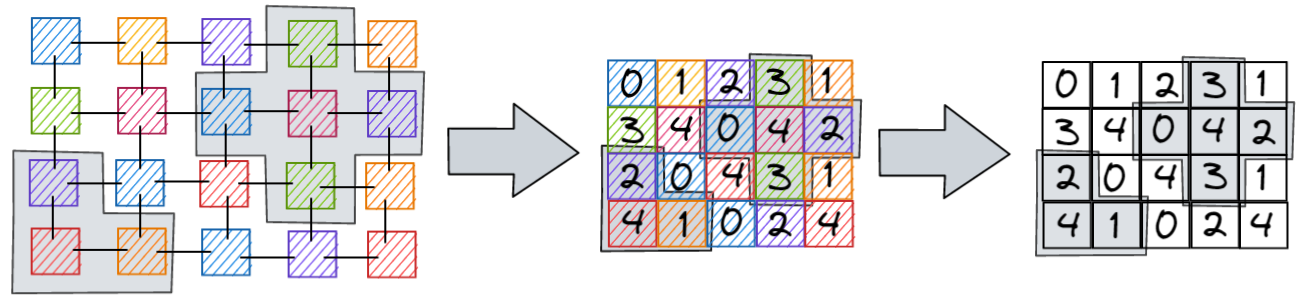
\includegraphics[width=1\textwidth]{Imagenes/ACaMatriz.PNG}
  \caption{Vecindades usuales para autómatas celulares}
  \label{fig:AC a matriz}
\end{figure}

Los elementos que definen a un autómata celular son:

\begin{itemize}
    \item Un espacio discreto $\mathcal{L}$ regular en el que se encuentran todas las células. En nuestro caso trabajaremos únicamente con espacios bidimensionales por lo que $\text{dim}(\mathcal{L})=m\times n$ para $m,n\in\mathbb{Z}$.
    \item Un conjunto finito $\Sigma$ de todos los posibles valores que pueda adquirir una célula. Cada elemento de $\Sigma$ se conocerá como un estado y cada célula podrá cambiar de estado en diferentes momentos del tiempo.
    \item Un sistema de vecindades que defina una topología sobre $\mathcal{L}$. Usualmente se define explícitamente la vecindad que se considera para todas las células.
    \item Una regla de evolución $\phi:\overbrace{\Sigma\times\Sigma\times\cdots\times\Sigma}^{N}\to\Sigma$ que define el cambio entre los $N$ posibles estados para una célula. Esta asignación puede tener componentes probabilísticos o ser completamente determinista, la manera en la que se defina esta regla dependerá completamente del fenómeno que se quiera modelar.
\end{itemize}

Así, podemos definir a un autómata celular en términos de sus elementos como una tupla, es decir, $A = (\mathcal{L}, \tau, \Sigma, \phi)$ es un autómata celular donde $\mathcal{L}$ es un espacio discreto y regular, $\tau$ es una topología definida a partir del sistema de vecindades que se establezca, $\Sigma$ es el conjunto de estados y $\phi$ la regla de evolución o cambios entre entados.

A continuación profundizaremos más sobre algunos de los conceptos que definimos en esta sección:

\subsection{Sistemas de vecindades}

Típicamente cuando se desarrollan análisis con autómatas celulares se trabaja con sistemas de vecindades definidos a partir de la vecindad de Moore o de la vecindad de Von neumann. Esta vecindad se compone de todas las células que rodean a la ubicada en alguna posición $i,j$ en nuestro espacio, la definimos como 

$$\mathcal{V}_M(x_{i,j}) = \{x_{k,l}||i-k|,|j-l|\leq1\text{, con }k,l\in\mathbb{Z}\}$$

Por otro lado encontramos a la vecindad de Von neumman, esta vecindad se compone de las celdas que rodean a la ubicada en la posición $i,j$ sin contar a los que se encuentran en las "esquinas". Se define como:

$$\mathcal{V}_V(x_{i,j}) = \{x_{k,l}||i-k|+|j-l|\leq1\text{, con }k,l\in\mathbb{Z}\}$$

\begin{figure}[h]
  \centering
    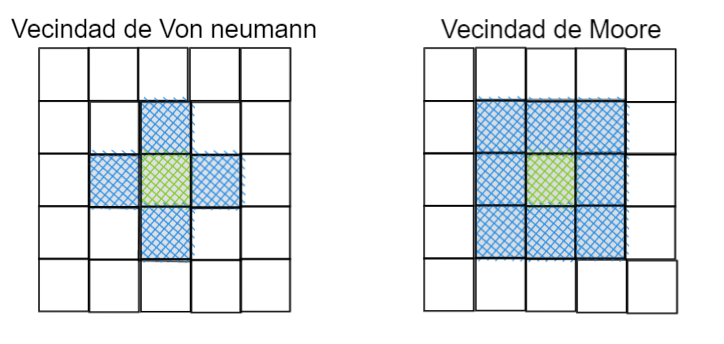
\includegraphics[width=0.6\textwidth]{Imagenes/vecindades.PNG}
  \caption{Vecindades usuales para autómatas celulares}
  \label{fig:Moore - Von neumann}
\end{figure}


